%%%%%%%%%%%%%%%%%%%%%%%
%% Folie             %%
%%%%%%%%%%%%%%%%%%%%%%%
\begin{frame}
    \frametitle{Goals Guided Research}

\begin{PraesentationAufzaehlung}
    \item Implementation of I2A
    \item 
\end{PraesentationAufzaehlung}

\end{frame}
\clearpage


%%%%%%%%%%%%%%%%%%%%%%%
%% Folie             %%
%%%%%%%%%%%%%%%%%%%%%%%
\begin{frame}
    \PraesentationUeberschriftZweizeilig{Imagination-Augmented Agent (I2A)}{Weber et al.(2017)}

\begin{PraesentationAufzaehlung}
    \item Architecture for deep reinforcement learning
    \item Imaginate the future and do better action based on this
    \item Combine model-free and model-based aspects
\end{PraesentationAufzaehlung}

\end{frame}
\clearpage

%%%%%%%%%%%%%%%%%%%%%%%%%%%%%%%%%%%%%%%%
%% Folie: Bilder - Zweispaltige Seite %%
%%%%%%%%%%%%%%%%%%%%%%%%%%%%%%%%%%%%%%%%
\begin{frame}
    \frametitle{I2A Architecture - Model Free Path}

\begin{multicols}{2}
	\begin{PraesentationAufzaehlung}
		\item Model Free Path
		\begin{itemize}
            \item Advantage-Actor-Critic (A2C)
        \end{itemize}
	    \item Model Based Path
		\begin{itemize}
			\item Imaginate the Future and use this information for desission making
		\end{itemize}
	\end{PraesentationAufzaehlung}
    \vfill\columnbreak
    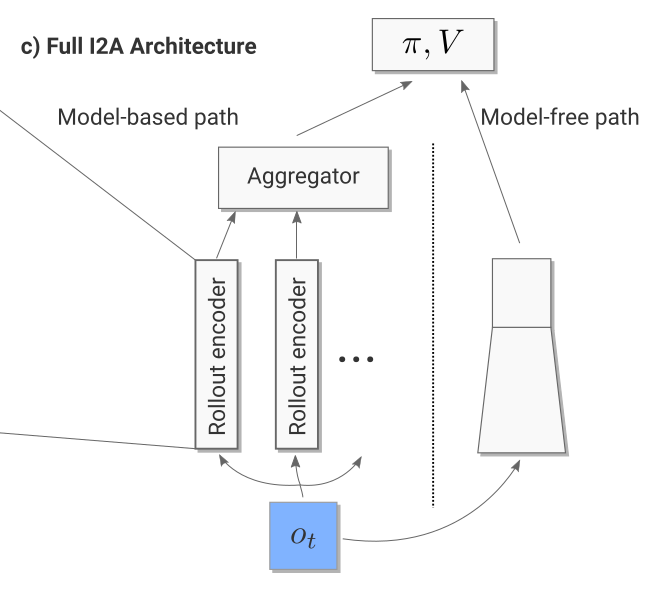
\includegraphics[width=\columnwidth, height=.7\textheight]{./Images/full_i2a_architecture.png}%
\end{multicols}
    
\end{frame}
\clearpage

%%%%%%%%%%%%%%%%%%%%%%%%%%%%%%%%%%%%%%%%
%% Folie: Bilder - Zweispaltige Seite %%
%%%%%%%%%%%%%%%%%%%%%%%%%%%%%%%%%%%%%%%%
\begin{frame}
    \frametitle{I2A Architecture - Model Based Path}

\begin{multicols}{2}
	\begin{PraesentationAufzaehlung}
	    \item Rollout encoder:\\
		Imaginate the Future and learn relevent information that can happen
		\item Aggregator: \\
		Concatitate the rollouts
	\end{PraesentationAufzaehlung}
    \vfill\columnbreak
    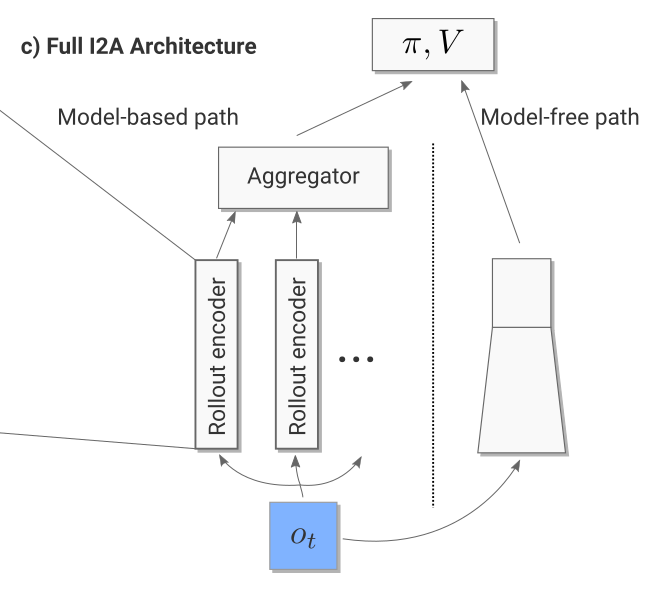
\includegraphics[width=\columnwidth, height=.7\textheight]{./Images/full_i2a_architecture.png}%
\end{multicols}
    
\end{frame}
\clearpage


%%%%%%%%%%%%%%%%%%%%%%%%%%%%%%%%%%%%%%%%
%% Folie: Bilder - Zweispaltige Seite %%
%%%%%%%%%%%%%%%%%%%%%%%%%%%%%%%%%%%%%%%%
\begin{frame}
    \frametitle{I2A Architecture - Imagination Rollout}

test
\begin{multicols}{2}
	\begin{PraesentationAufzaehlung}
		\item Imagine Future:\\
		Rollout the future for an input observation
	    \item Imagination Core:\\
		Imaginate the next observation $o_{t+i}$ and the next reward $r_{t+i}$
	\end{PraesentationAufzaehlung}
    \vfill\columnbreak
    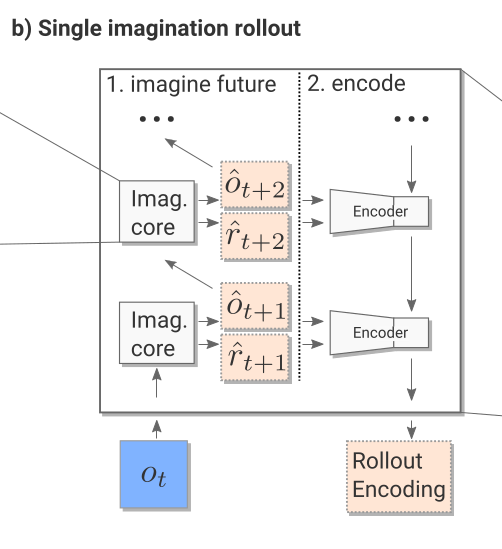
\includegraphics[width=\columnwidth]{./Images/single_imagination_rollout.png}%
\end{multicols}
    
\end{frame}
\clearpage

%%%%%%%%%%%%%%%%%%%%%%%%%%%%%%%%%%%%%%%%
%% Folie: Bilder - Zweispaltige Seite %%
%%%%%%%%%%%%%%%%%%%%%%%%%%%%%%%%%%%%%%%%
\begin{frame}
    \frametitle{I2A Architecture - Imagination Rollout}

\begin{multicols}{2}
	\begin{PraesentationAufzaehlung}
		\item Encoder:\\
		CNN Network followed by an LSTM Network\\
		Learns usefull information from the rollouts
	\end{PraesentationAufzaehlung}
    \vfill\columnbreak
    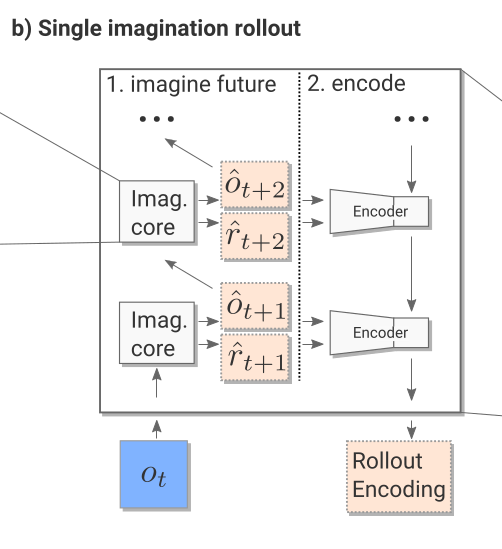
\includegraphics[width=\columnwidth]{./Images/single_imagination_rollout.png}%
\end{multicols}
    
\end{frame}
\clearpage

%%%%%%%%%%%%%%%%%%%%%%%%%%%%%%%%%%%%%%%%
%% Folie: Bilder - Zweispaltige Seite %%
%%%%%%%%%%%%%%%%%%%%%%%%%%%%%%%%%%%%%%%%
\begin{frame}
    \frametitle{I2A Architecture - Imagination Core}

\begin{multicols}{2}
	\begin{PraesentationAufzaehlung}
	    \item Imaginate the next observation $o_{t+i}$ and the next reward $r_{t+i}$
		\item policy network $\pi$\\
		desides the next action $a_t$
		\item environment model EM imaginate what will happen if we are in state $o_t$ and do action $a_t$
	\end{PraesentationAufzaehlung}
    \vfill\columnbreak
    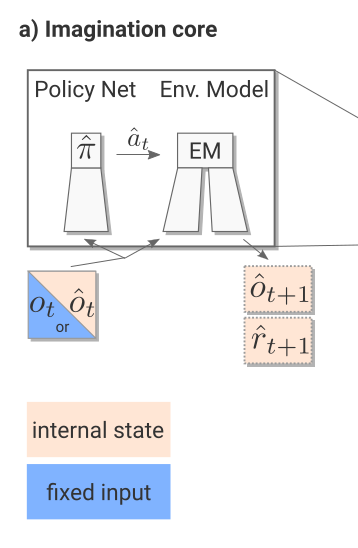
\includegraphics[height=0.7\textheight]{./Images/Imagination_core.png}%
\end{multicols}
    
\end{frame}
\clearpage





